\tikzstyle{edge}=[black, thick, draw]
\tikzstyle{arr}=[black, thick, draw, <->]
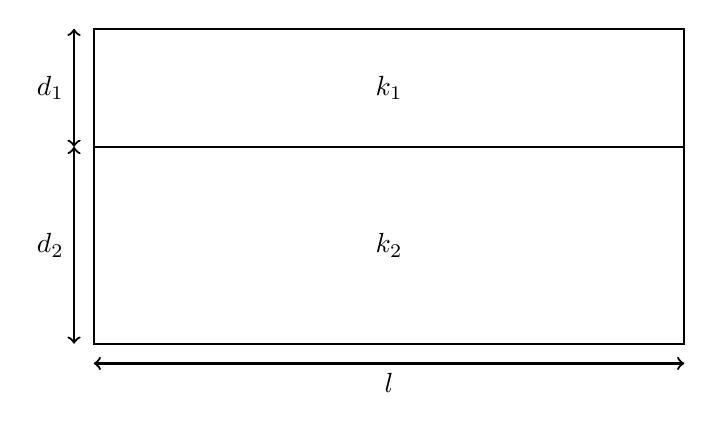
\begin{tikzpicture}[scale=0.5]
  \draw [edge] (0,0) -- (15,0) -- (15,5) -- (0,5) -- cycle;
  \draw [edge] (0,5) -- (15,5) -- (15,8) -- (0,8)  -- cycle;
  \draw [arr] (0,-0.5) -- (15,-0.5) node[midway, below]{$l$};
  \draw [arr] (-0.5,0) -- (-0.5,5) node[midway, left]{$d_2$};
  \draw [arr] (-0.5,5) -- (-0.5,8) node[midway, left]{$d_1$};

  \node (k2) at (7.5,2.5) {$k_2$};
  \node (k1) at (7.5,6.5) {$k_1$};
\end{tikzpicture}


